\documentclass[12pt]{rockefeller}
\usepackage[pdftex]{graphicx} 
\graphicspath{{/Users/tasos/Desktop/strasbourg_05_2017/}} %directory of figures
\usepackage[english]{babel} %set language
\usepackage{helvet} %set font to Helvetica
\renewcommand\familydefault{\sfdefault} %set font to Helvetica
\usepackage{fancyhdr} %header and footer
\usepackage[utf8x]{inputenc} %allow greek input
\usepackage[LGR,T1]{fontenc} %allow greek input
\newcommand{\textgreek}[1]{\begingroup\fontencoding{LGR}\selectfont#1\endgroup} %allow greek input
\usepackage{hyperref} %allow hypertexting
\usepackage[acronym,xindy,toc]{glossaries} %glossary 
\makeglossaries %glossary 
\usepackage[xindy]{imakeidx} %glossary 
\makeindex %glossary 



%\usepackage{enumerate}
%\usepackage{threeparttable}
%\usepackage{multirow}
%\usepackage[algoruled,linesnumbered,lined]{algorithm2e}
%\usepackage[font=footnotesize,caption=false]{subfig}
%\usepackage{amssymb}
%\usepackage{amsmath}
%\usepackage[pdftex,bookmarks=true]{hyperref}
%\newcommand{\subsubsubsection}[1] {\noindent {\underline {#1}}}
\newcommand{\snp}[1] {\noindent {\underline {#1}}}

\begin{document}

\author{Tasos Gogakos}
\title{\MakeUppercase{Characterizing human transfer rnas by hydro-trnaseq and par-clip}}
\date{June 2017}

\maketitle

\thispagestyle{empty}
\makecopyright


\begin{abstract}

The participation of \glspl{trna} in fundamental aspects of biology and disease necessitates an accurate, experimentally confirmed annotation of tRNA genes, and curation of precursor and mature tRNA sequences. This has been challenging, mainly because RNA secondary structure and nucleotide modifications, together with tRNA gene multiplicity, complicate sequencing and sequencing read mapping efforts. To address these issues, we developed hydro-tRNAseq, a method based on partial alkaline RNA hydrolysis that generates fragments amenable for sequencing. To identify transcribed tRNA genes, we further complemented this approach with Photoactivatable Crosslinking and Immunoprecipitation (PAR-CLIP) of SSB/La, a conserved protein involved in pre-tRNA processing. Our results show that approximately half of all predicted tRNA genes are transcribed in human cells. We also report predominant nucleotide modification sites, their order of introduction, and identify tRNA leader, trailer and intron sequences. By using complementary sequencing-based methodologies we present a human tRNA atlas, and determine expression levels of mature and processing intermediates of tRNAs in human cells.
\end{abstract}


%Dedication
\chapter*{} %blank chapter, no title, not included in table of contents
\addtocounter{page}{2} %fix numbering
\vspace{3in} %start the dedication close to the bottom of page
\begin{flushright} %center everything
\emph{\textgreek{Stous gone'is kai ton aderf'o mou}}
\end{flushright}

\chapter*{Acknowledgments} %uncounted chapter

First, I would like to thank my  

\renewcommand\contentsname{Table of Contents}
\tableofcontents
\cleardoublepage
\phantomsection
\addcontentsline{toc}{chapter}{List of Figures}
\listoffigures
\cleardoublepage
\phantomsection
\addcontentsline{toc}{chapter}{List of Tables}
\listoftables

%glossary
\newacronym[plural=tRNAs, firstplural=transfer RNAs]{trna}{tRNA}{transfer RNA}
\printglossary[type=\acronymtype,nonumberlist,title={List of Abbreviations}]

%----------
%mainmatter
%----------
\mainmatter
\pagestyle{fancy}
\fancyhf{}
\lhead{\chaptername\ \thechapter}
\rhead{\thesection}
\rfoot{\thepage}

\chapter{Introduction}
\section{New section}

\begin{figure}[!ht]%
\centering
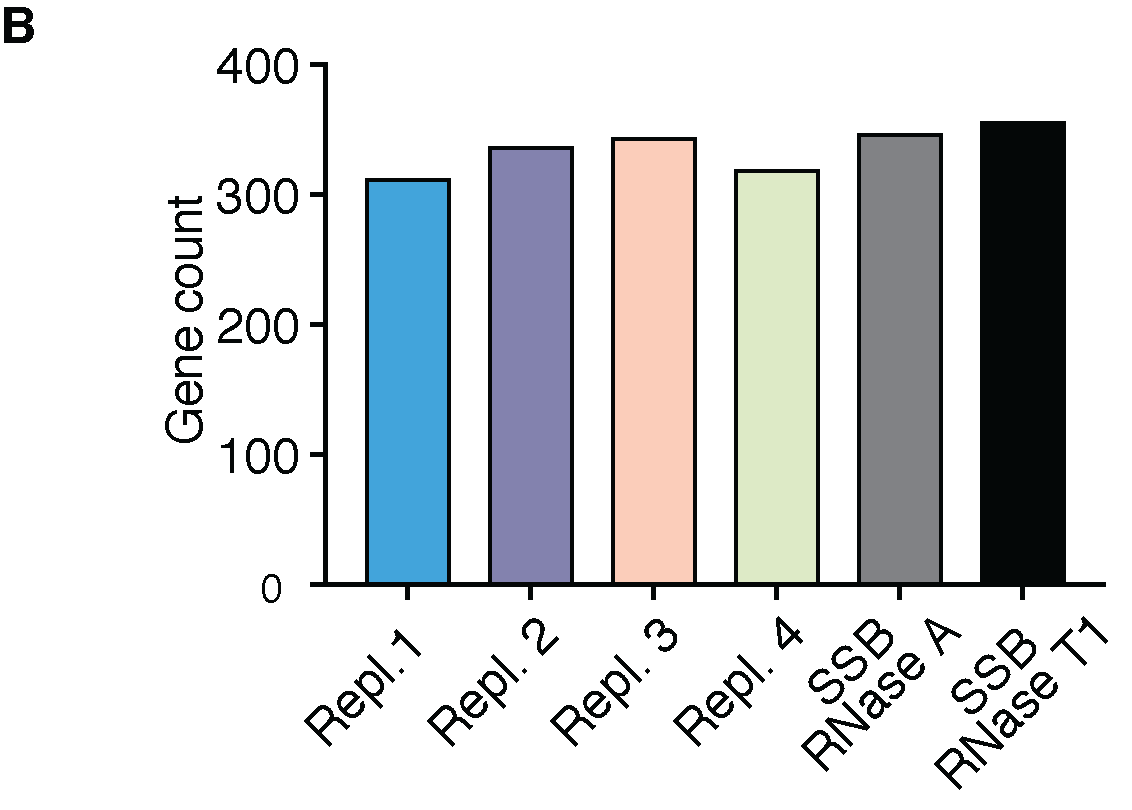
\includegraphics[width=3.5in]{venn_bars.png}%
\caption{Venn Bars}%
\label{fVenn}%
\end{figure}

\newpage

\cite{Arimbasseri:2016ey}
\chapter{woohooo}
this is a new chapter\newpage
this is pager 2

\newpage
\renewcommand{\bibname}{References}
\bibliographystyle{IEEEtran}
\bibliography{./tasos_v1.bib}
\phantomsection
\addcontentsline{toc}{chapter}{References} %rename references

\end{document}
